%%%%%%%%%%%%%%%%%%%%%%%%%%%%%%%%%%%%%%%%%%%%%%%%%
\newpage
%%%%%%%%%%%%%%%%%%%%%%%%%%%%%%%%%%%%%%%%%%%%%%%%%

\subsection{weitere Diagramme}


\sa{own: Bild tauschen}
\begin{figure}[hptb]
 \centering
 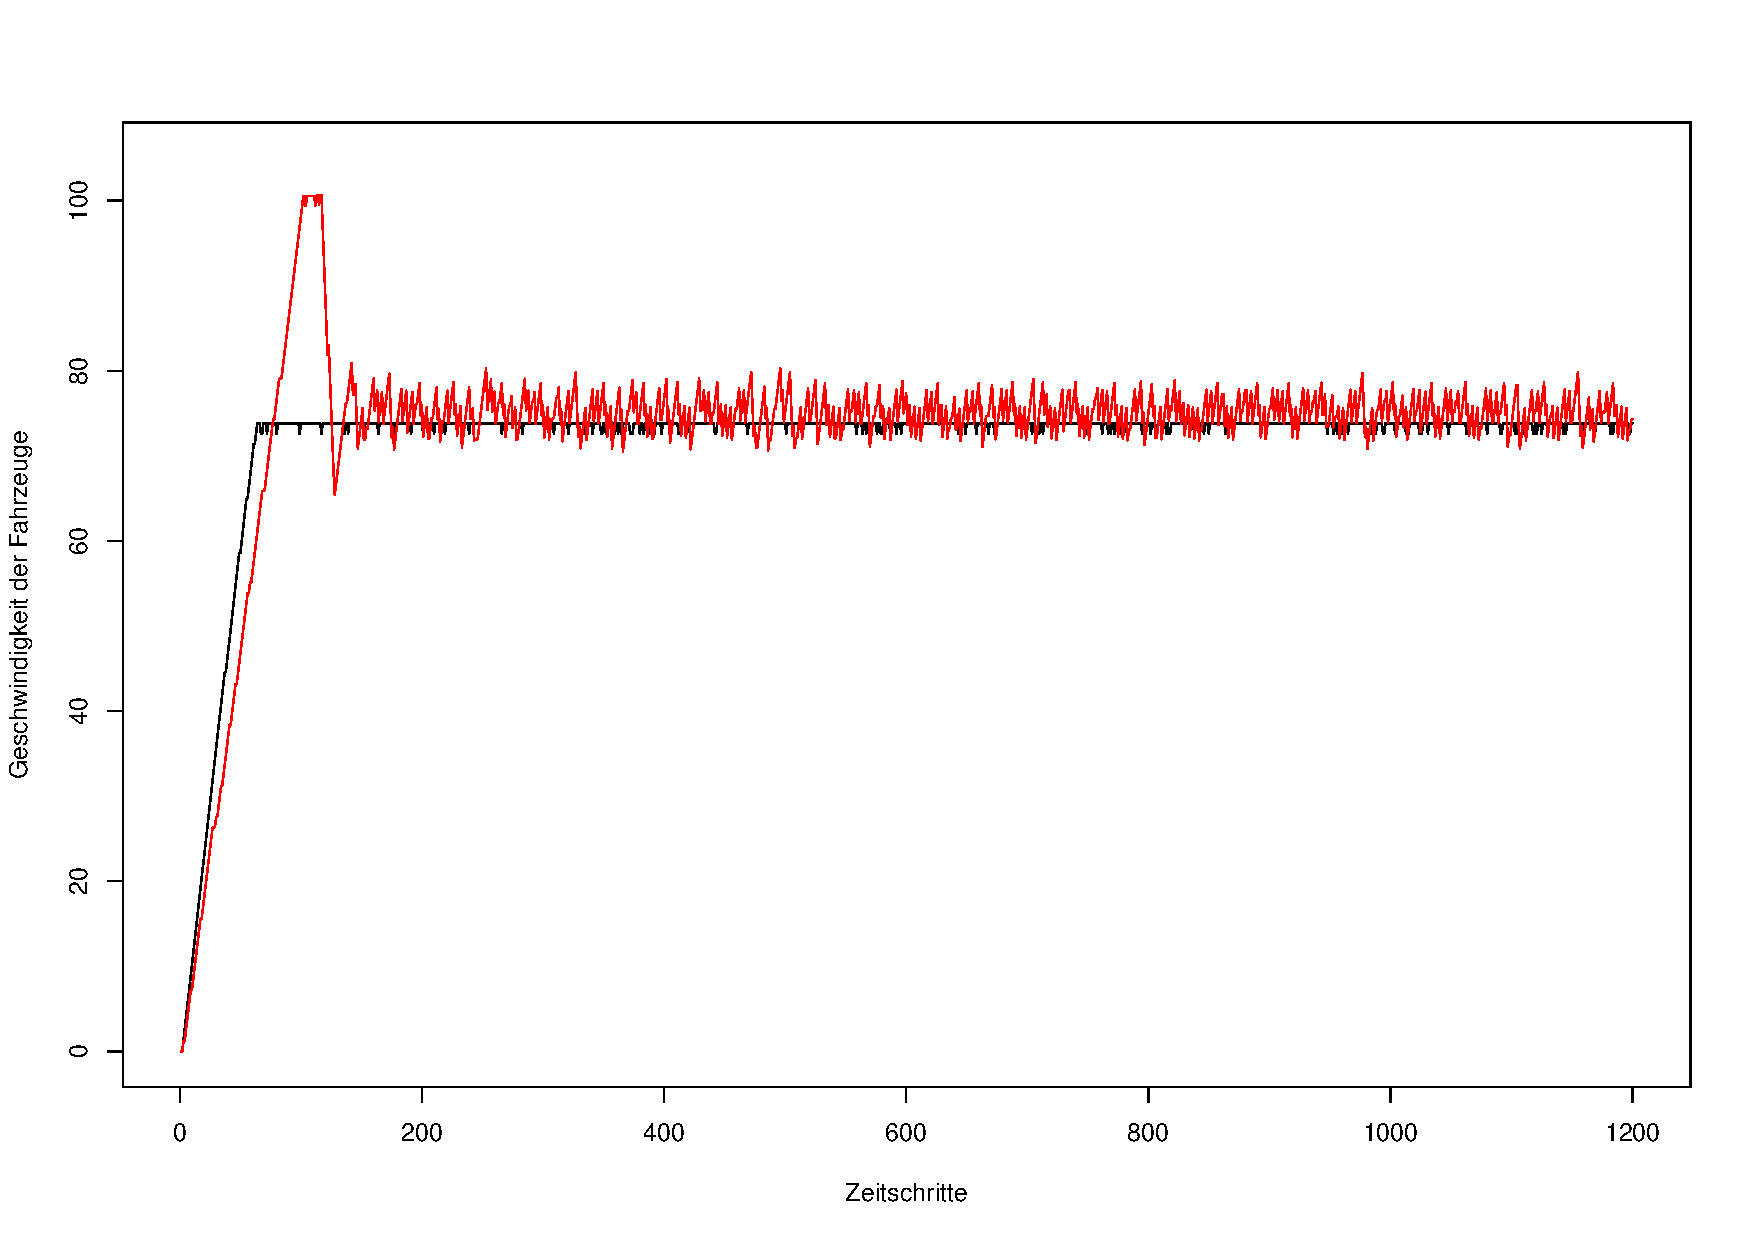
\includegraphics[width=0.95\textwidth]{speed_run27}
 \caption[kurzText]
 		{Positionsdiagram}
 \label{figure:33veh-1km}
\end{figure}

\cref{figure:33veh-1km} entstand aufgrund einer Fehleinstellung in der Szenariodatei.
Hier fuhren 33 Fahrzeuge auf einer Strecke von 1 km.
\\
Zu Beginn sieht man aufgrund der enger werdenden Punktmuster, dass sich die Geschwindigkeit der Fahrzeuge nur verlangsamt. Dann kommt es zu einer länger anhaltenden Stillstandsphase der Fahrzeuge, die auch zu Simulationsende noch anhielt.
\\
Hier erkennt man die in den Versuchen in \cite{na-sch} erkannte Rückwärtsbewegung der Stauwelle.







%%%%%%%%%%%%%%%%%%%%%%%%%%%%%%%%%%%%%%%%%%%%%%%%%

	%   %	%   %	 %%%%	%%%%%	%%%%%	%%%%
	%% %%	%   %	%		  %		%		%   %
	% % %	%   %	 %%%	  %		%%%		%%%%
	%   %	%   %	    %	  %		%		%  %
	%   %	 %%%	%%%%	  %		%%%%%	%	%

%%%%%%%%%%%%%%%%%%%%%%%%%%%%%%%%%%%%%%%%%%%%%%%%%

\begin{figure}[hptb]
 \centering
 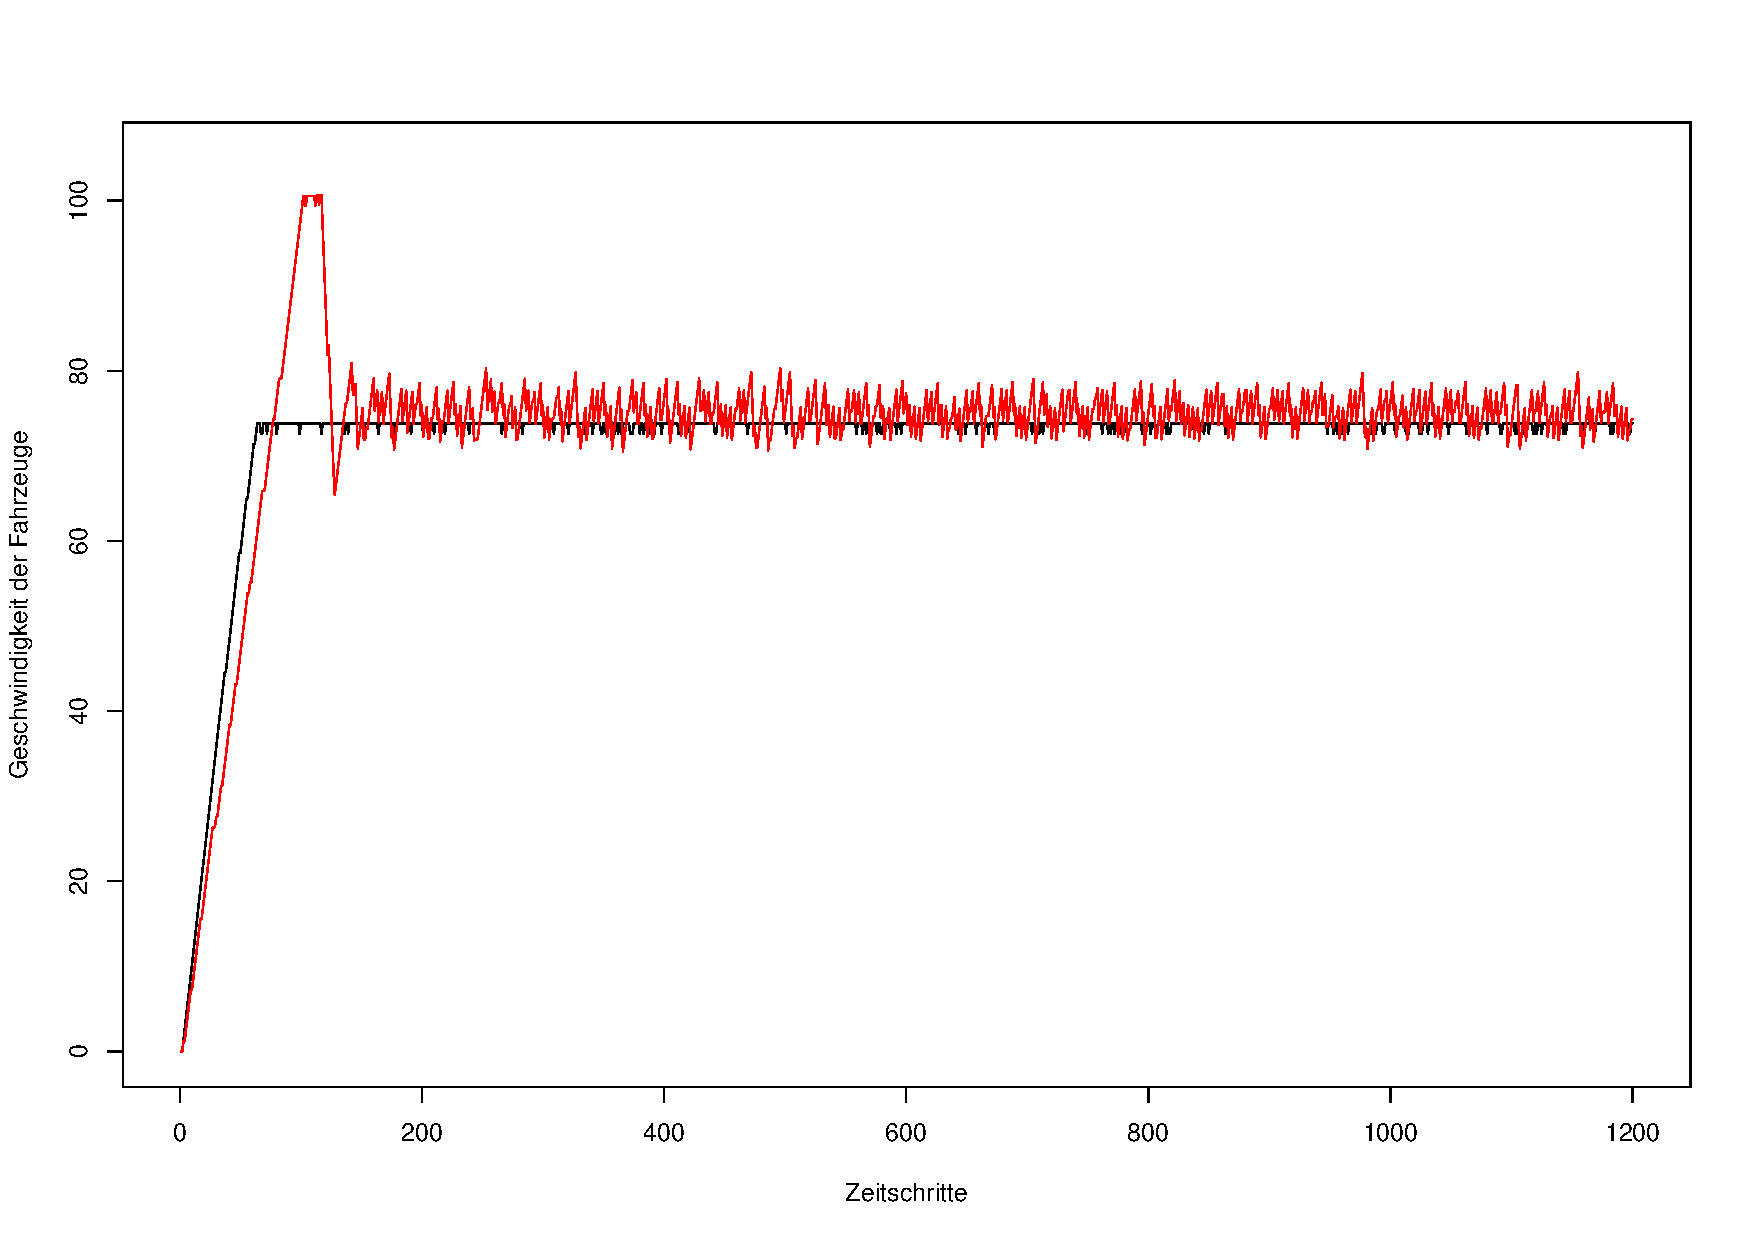
\includegraphics[width=0.9\textwidth]{speed_run27}
 \caption[kurzText]
 		{Text}
 \label{figure:image1}
\end{figure}


\begin{figure}[hptb]
  \centering 
   \subfigure[Text1]{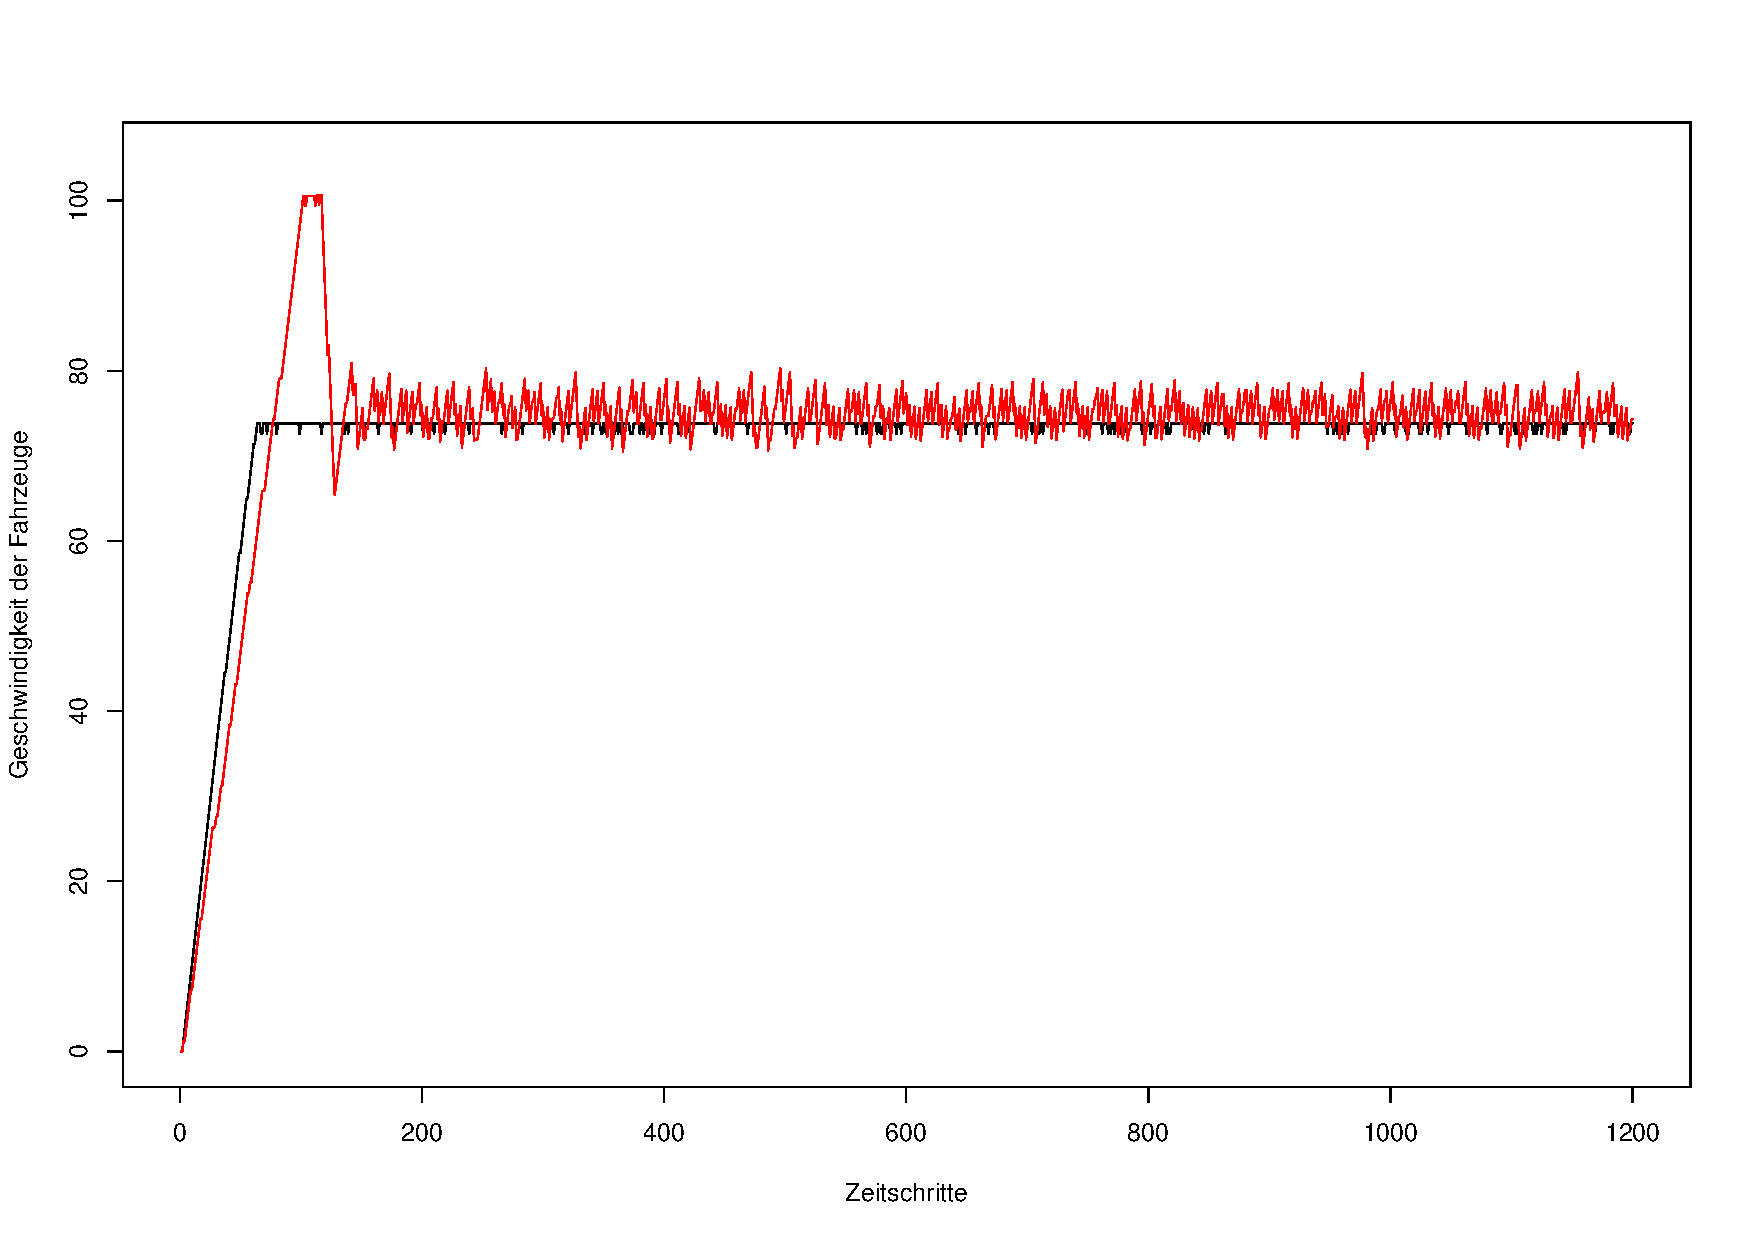
\includegraphics[width=0.45\textwidth]{speed_run27}\label{figure:image2-1}}\qquad 
   \subfigure[Text2]{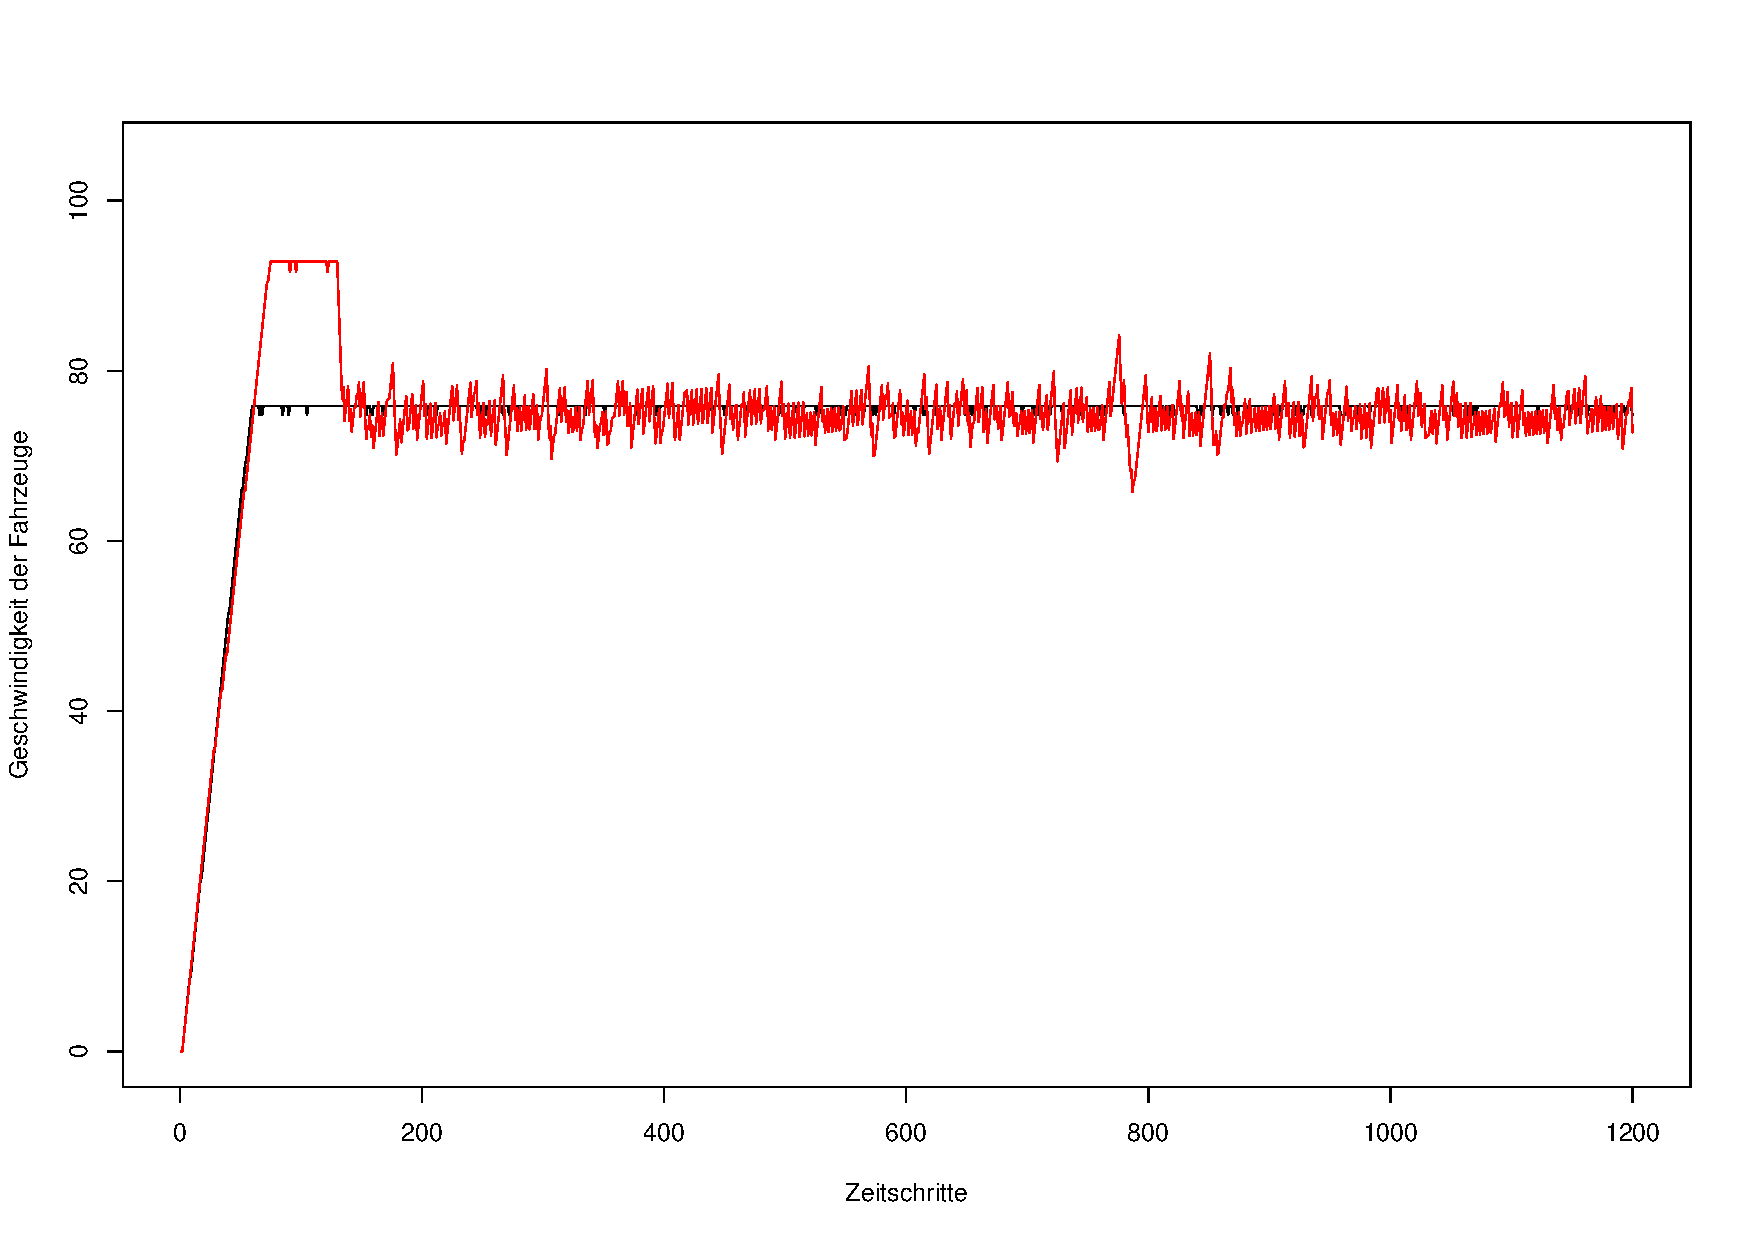
\includegraphics[width=0.45\textwidth]{speed_run28}\label{figure:image2-2}}  \caption{Text} 
  \label{figure:image2}
\end{figure}


\begin{figure}[hptb]
  \centering 
   \subfigure[Text1]{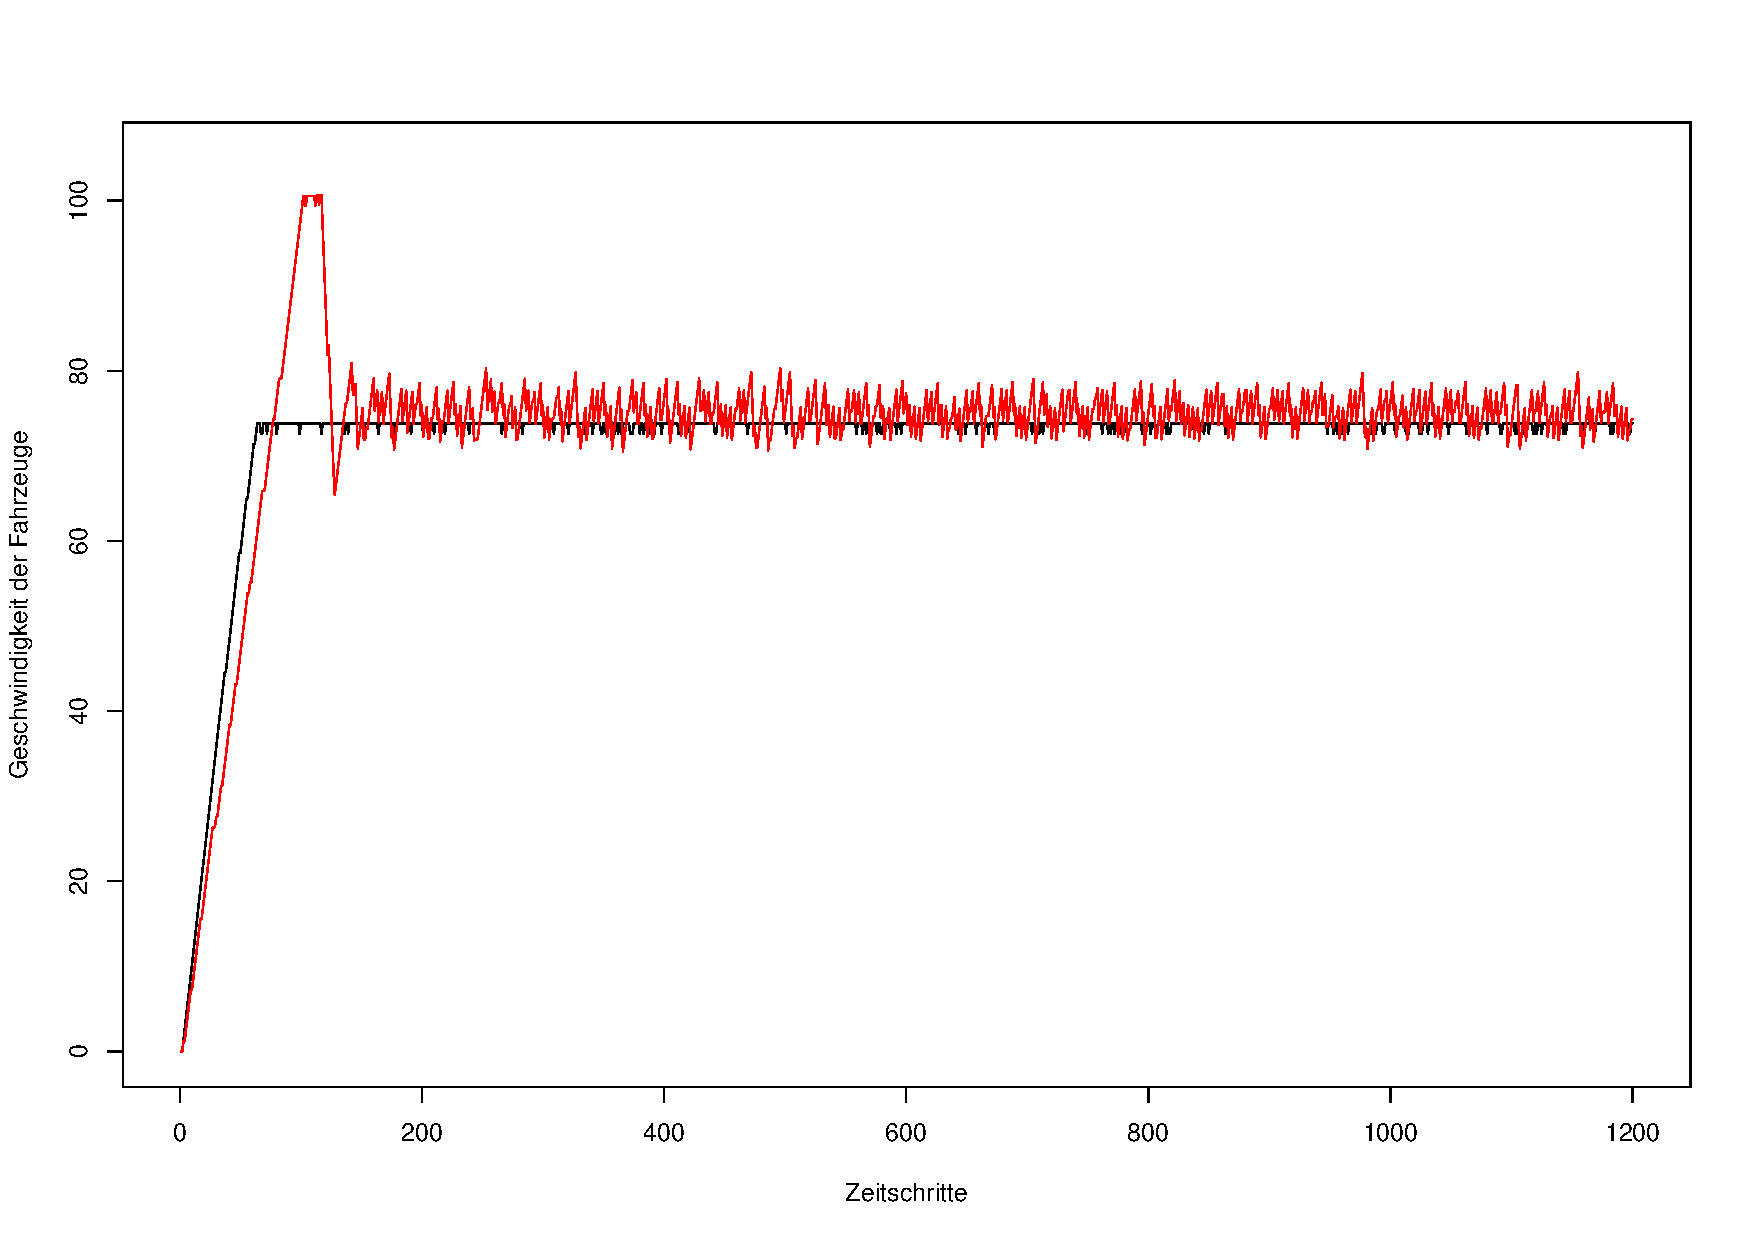
\includegraphics[width=0.3\textwidth]{speed_run27}\label{figure:image3-1}}\qquad 
   \subfigure[Text2]{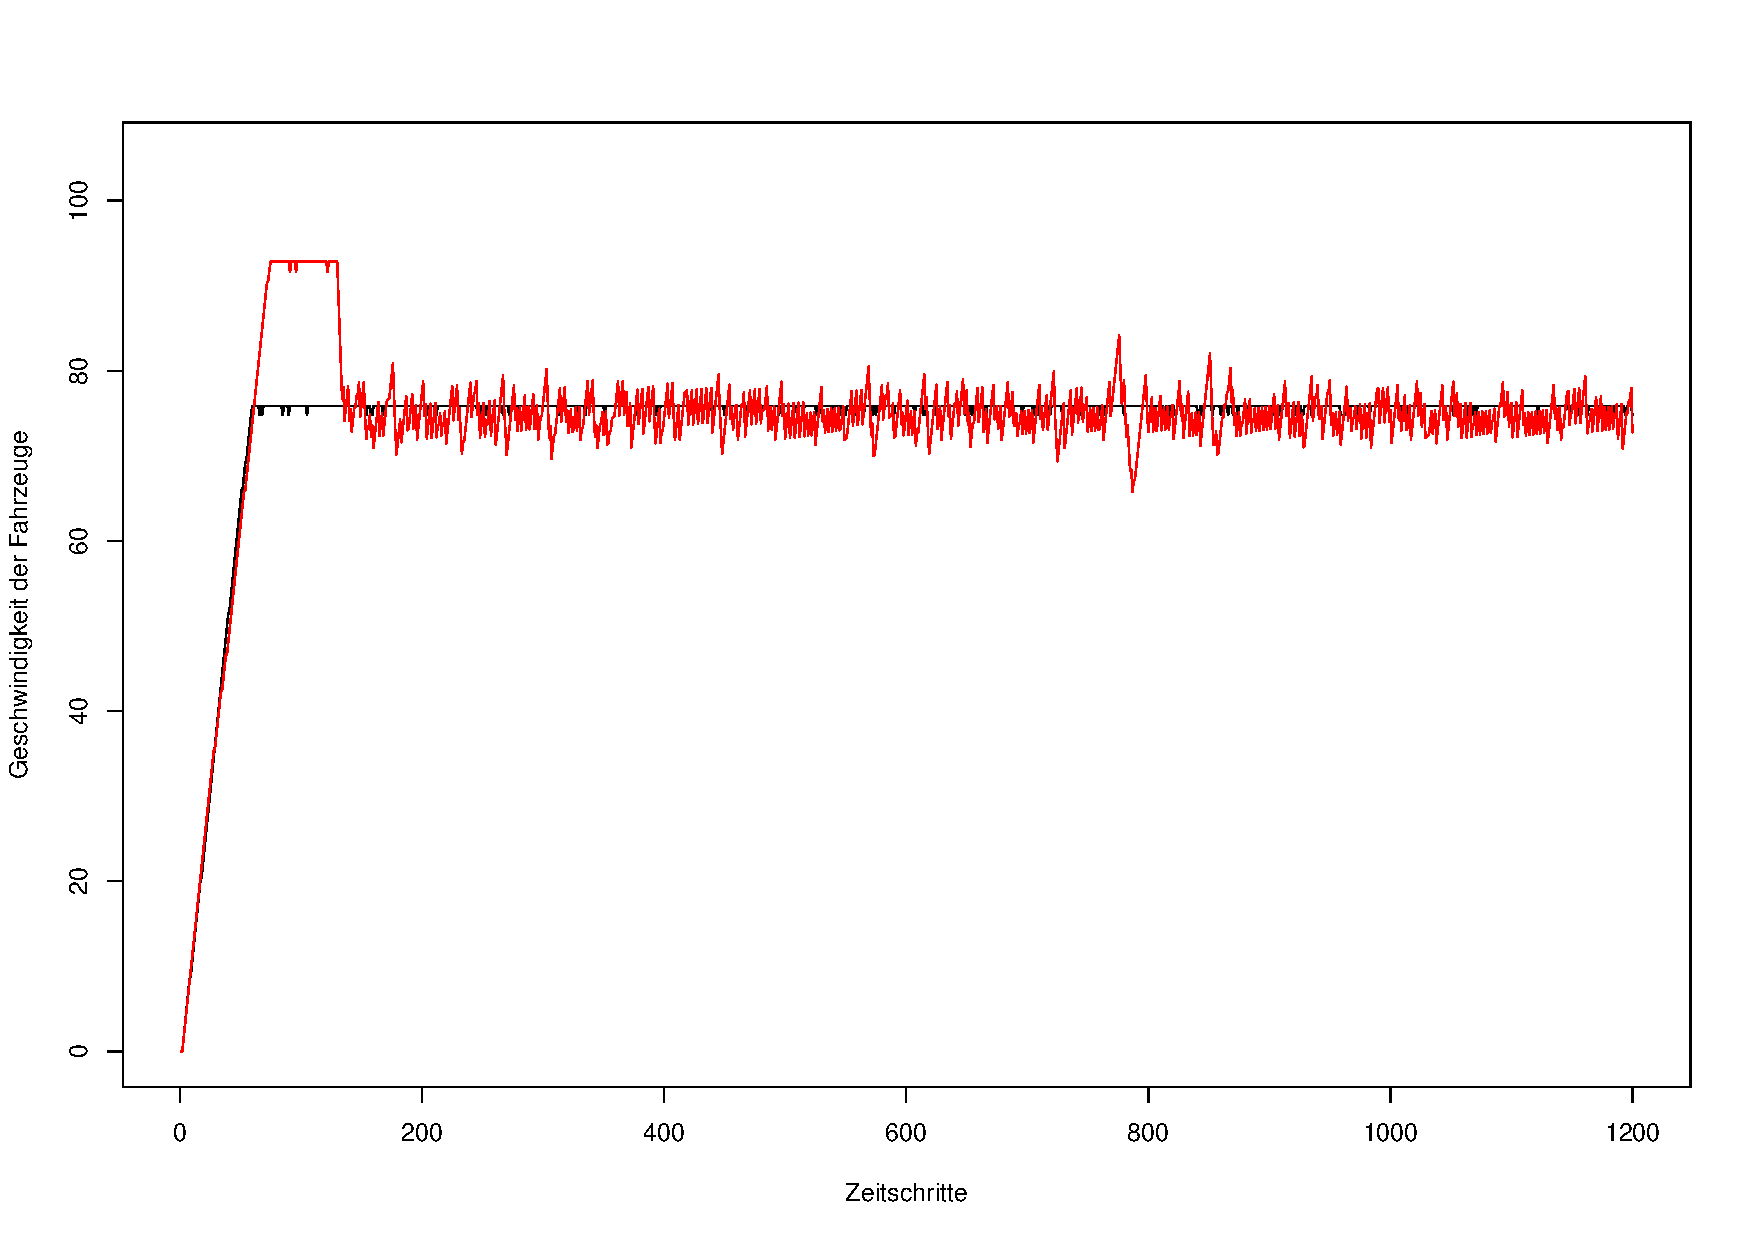
\includegraphics[width=0.3\textwidth]{speed_run28}\label{figure:image3-2}}\qquad 
   \subfigure[Text3]{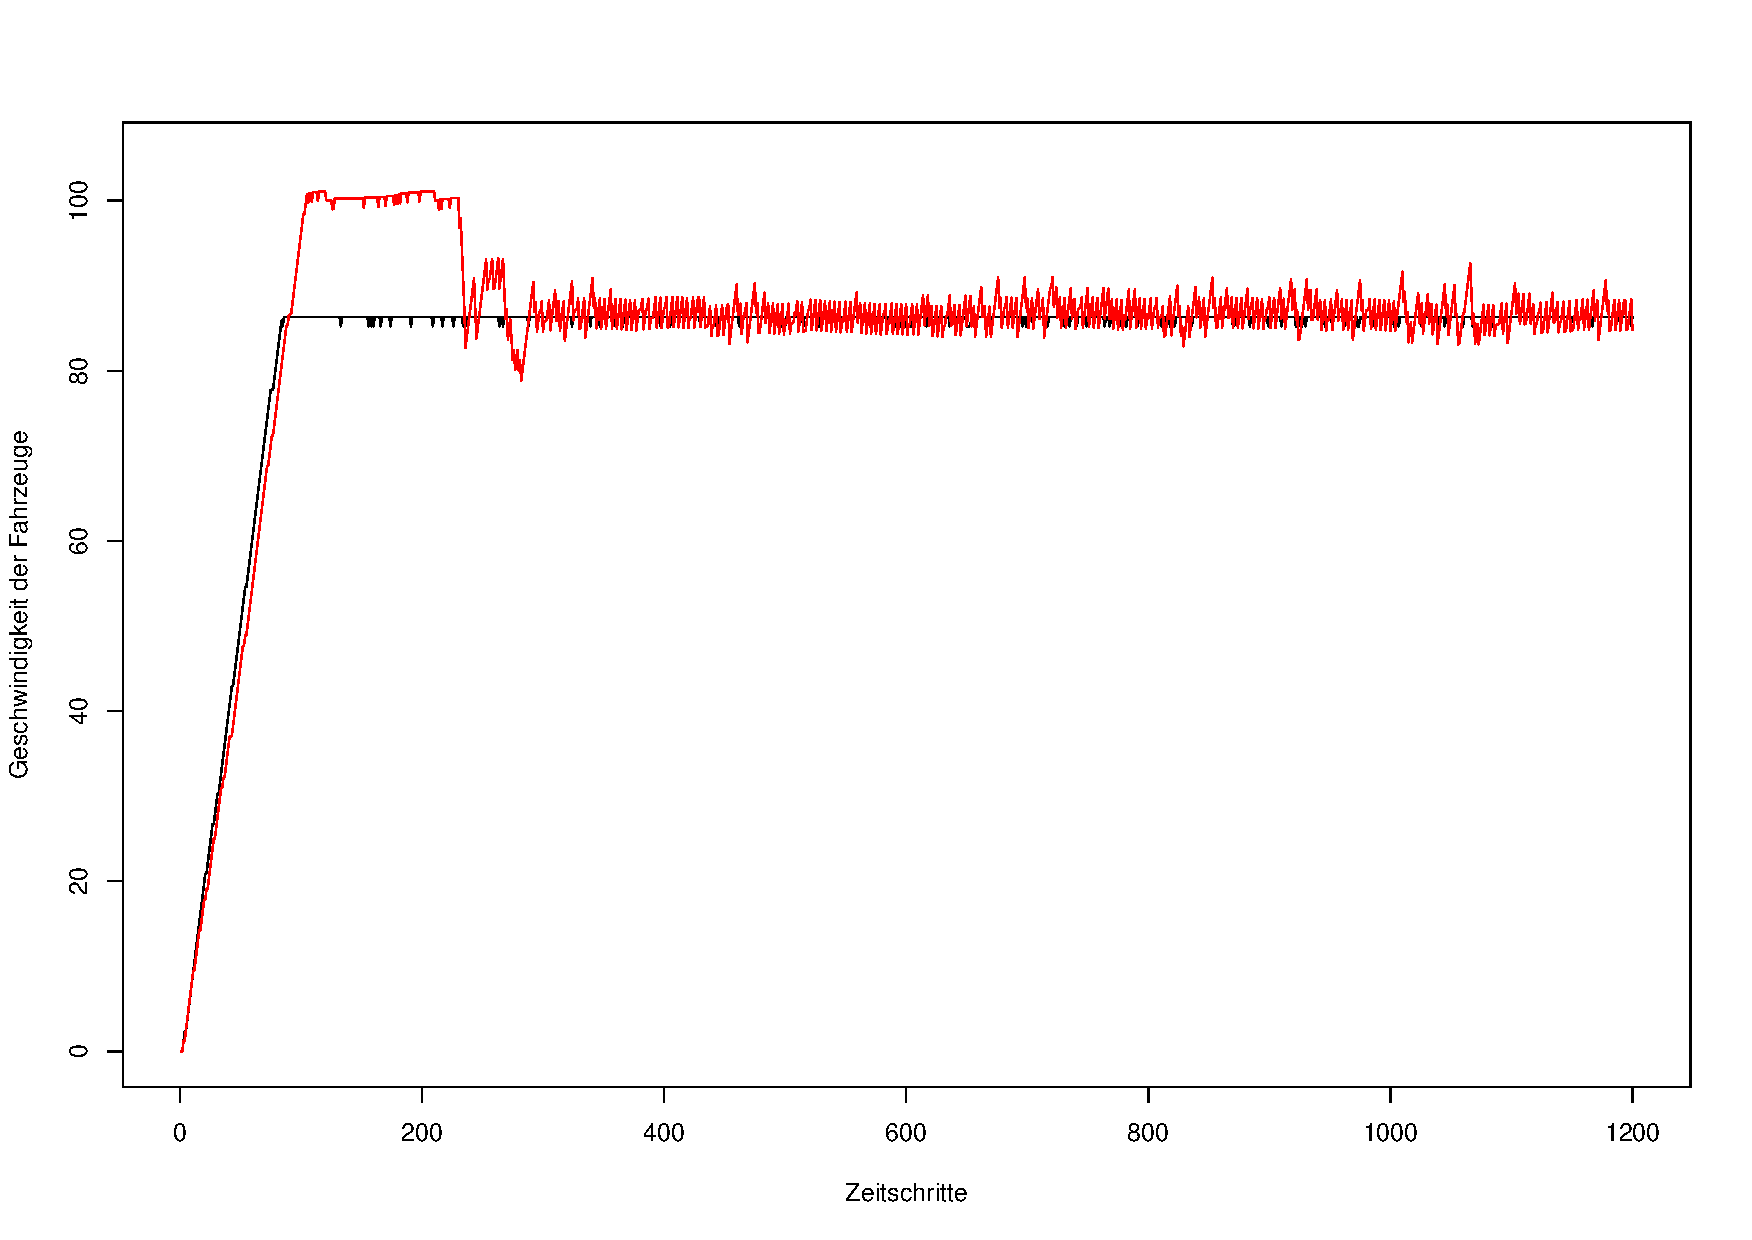
\includegraphics[width=0.3\textwidth]{speed_run29}\label{figure:image3-3}}
  \caption{Text} 
  \label{figure:image3}
\end{figure}

